% The "%" character denotes a comment
% This file was written by Nathan Moore, Winona State University
% as a template for how lab reports might be written in LaTeX.
% style choices originally come from the American Journal of Physics's
% sample submission file, http://ajp.dickinson.edu/Contributors/manFormat.html
%
%
\documentclass[prb,preprint]{revtex4-1}
\usepackage{amsmath}  % needed for \tfrac, \bmatrix, etc.
\usepackage{amsfonts} % needed for bold Greek, Fraktur, and blackboard bold
\usepackage{graphicx} % needed for figures

%these are some macros (shortcuts)
\newcommand{\bea}{\begin{eqnarray}}
\newcommand{\eea}{\end{eqnarray}}
\newcommand{\be}{\begin{equation}}
\newcommand{\ee}{\end{equation}}

\begin{document}

\title{Electronics Lab 05: Analogue to Digital Converters}
\author{Adam Stammer}
%\email{adam.stammer@go.winona.edu}

\date{\today}

%if you include an abstract, it goes here
\begin{abstract}
We introduced comparators as a new integrated circuit and applied them in a digital to analogue converter (ADC), a very common and useful circuit. Our ADCs successfully turned an incoming signal, alternating or otherwise, into a respective $2^{n}-1$ format binary output. Using 4 comparators we achieved a 4 bit output, but only used 5 potential outputs. To further this design we could build a code converter to turn our 4 bit $2^{n}-1$ where n = the number of bits + 1, signal into a standard binary signal.
\end{abstract}

\maketitle


%These are my general reccomendations for an undergraduate lab report in Physics. 
%
%\textbf{Purpose}
%The lab report should start with a purpose statement.  Briefly 
%provide the necessary background and explain what problem your are trying to 
%solve/investigate.
%
%\textbf{Conclusions} Don't be coy, cut to the point right away and state what you found. This should be breif.
%
%\textbf{Theory} We never just measure stuff in Physics.  There's always a 
%theoretical idea behind the measurement we're making.  Explain  the ideas 
%behind your work, starting at the level of a successful Physics 221/222 
%student.
%
%\textbf{Data} Sketch out, in words and pictures, the apparatus you used to take data.  Report the data, graphically, if possible, and state the uncertainties  in your measurement.  Don't provide pages of computer printout here. Data tables shouldn't be your first choice when it comes to communicating your measurements.\cite{Tufte}
%
%\textbf{Analysis} With data presented, describe how the theory agrees/disagrees with 
%the data you took.  Normally this is accomplished with a fit line (or math 
%model) that is interpreted.
%
%\textbf{Limitations and Recommendations} Every measurement has limitations and it is only honest to report them to the reader.  ``Human Error'' is a meaningless statement.  After your analysis is complete, revisit the purpose statement.  This is the place to more forcefully argue your conclusions.    
%
%Notes: 
%Writing in the first person, eg ``I" or ``We," is fine.
%
%\newpage
%\textbf{Example Lab Report:}

\section{Purpose}
To familiarize ourselves with comparators as a standardized circuit and apply them in a meaningful way. Conversion from analogue to digital, and back, is one of the most common electronic hardware applications. While we didn't go in depth into the world of ADCs, we now have a basic understanding of one way they can work and this gave us a practical use case of comparators.

\section{Conclusions}
A comparator based ADC is relatively simple in design but rather costly in both hardware and space. Each comparator adds only one additional layer of accuracy, not even an entire bit. It's rare that such a design would be practical in any format other than an integrated circuit. Nonetheless, our design did indeed work and it is directly scalable.

\section{Theory}
We can set each comparator to turn on an led when Vin is greater than Vref with the rather simple circuit diagram seen below.

\begin{figure}[ht]
\centering
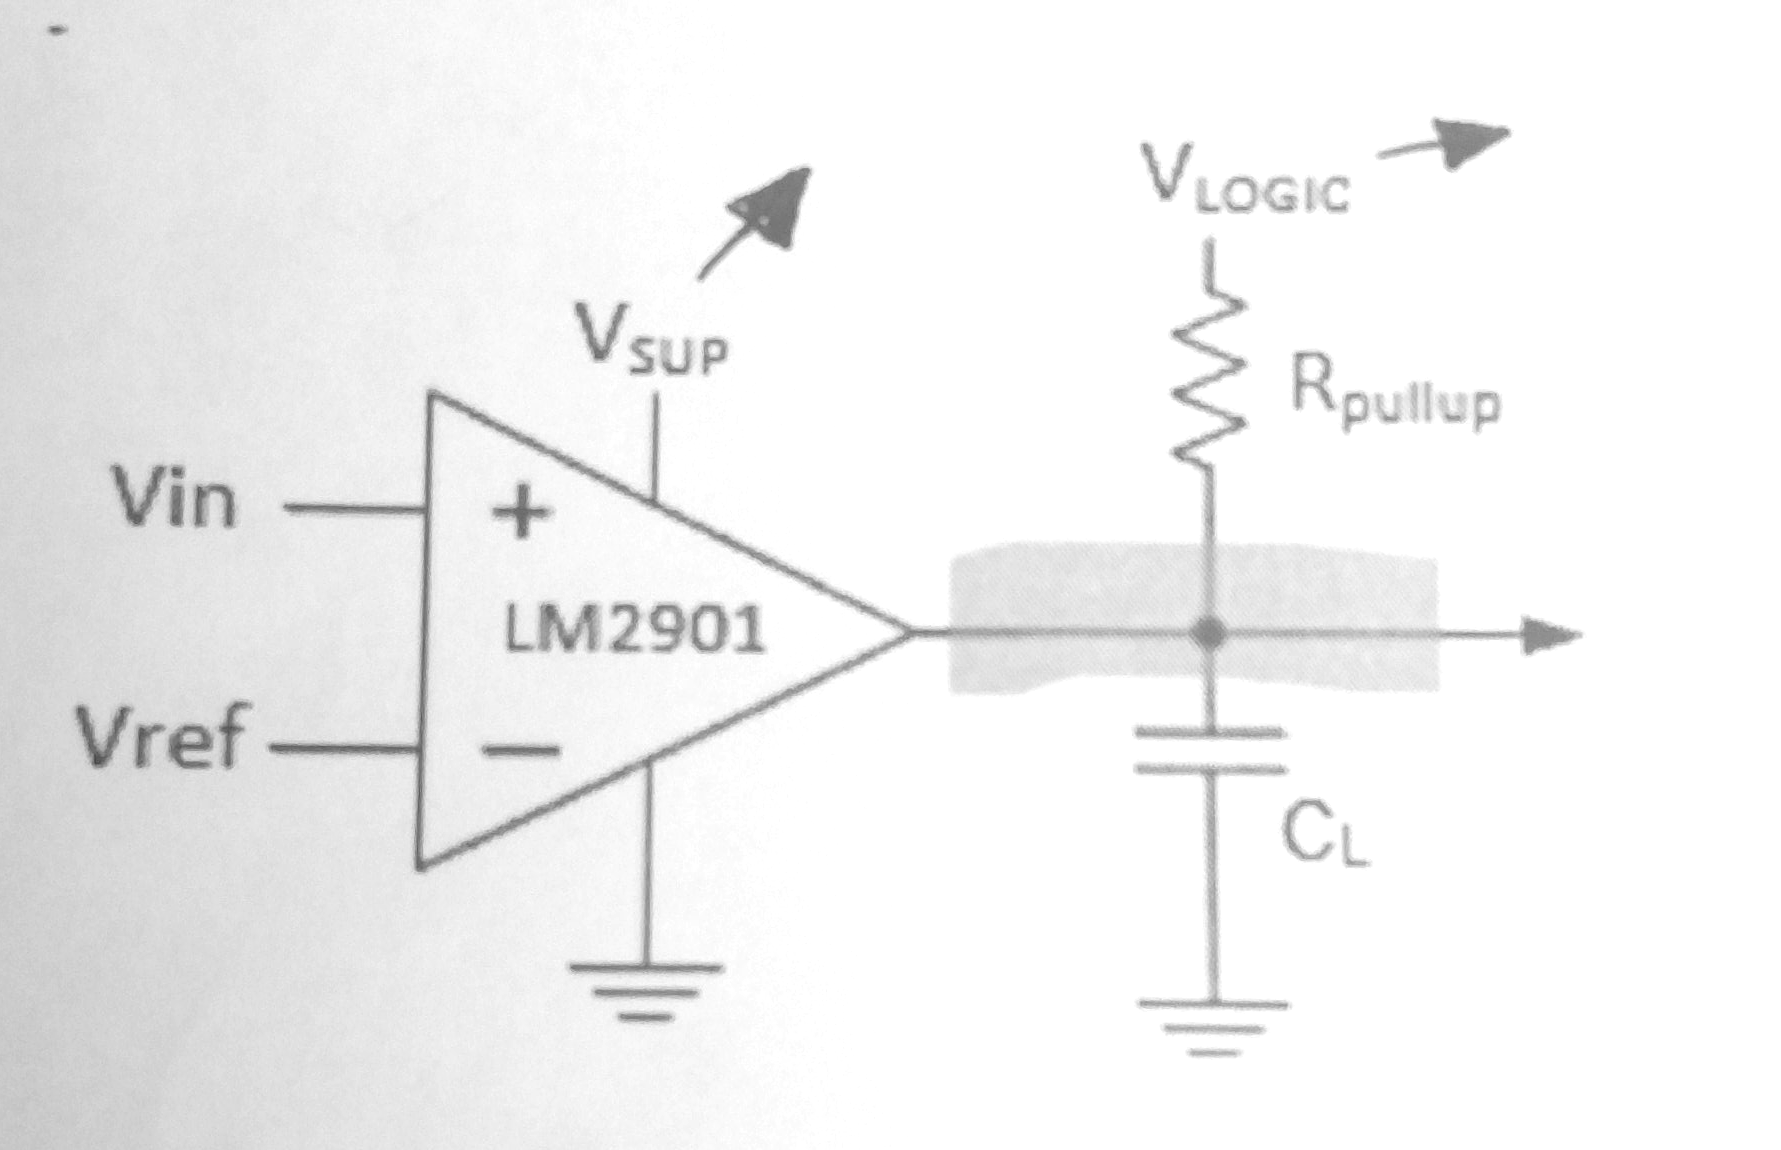
\includegraphics[width=4in]{schem.png}
\caption{Frequency and Gain Voltages}
\label{fig1}
\end{figure}

If we can build a linear increasing Vref, we can use the same Vin and multiple comparators, one for each led, to achieve a shifting binary output of signal amplitude. Since comparators have a very high input impedance we can use simple voltage dividers to achieve our varying Vref values, and a "ladder" resistor will save us some space and building complexity as well.

Below you can see a circuit diagram implementing 4 comparators, one for each led and reference voltage. Note that $V_{sup}$ must be at least 2 Volts above $V_{logic}$, since we are using the LM239 comparators. That makes this design quite simple to scale, although not very space efficient.

\begin{figure}[ht]
	\centering
	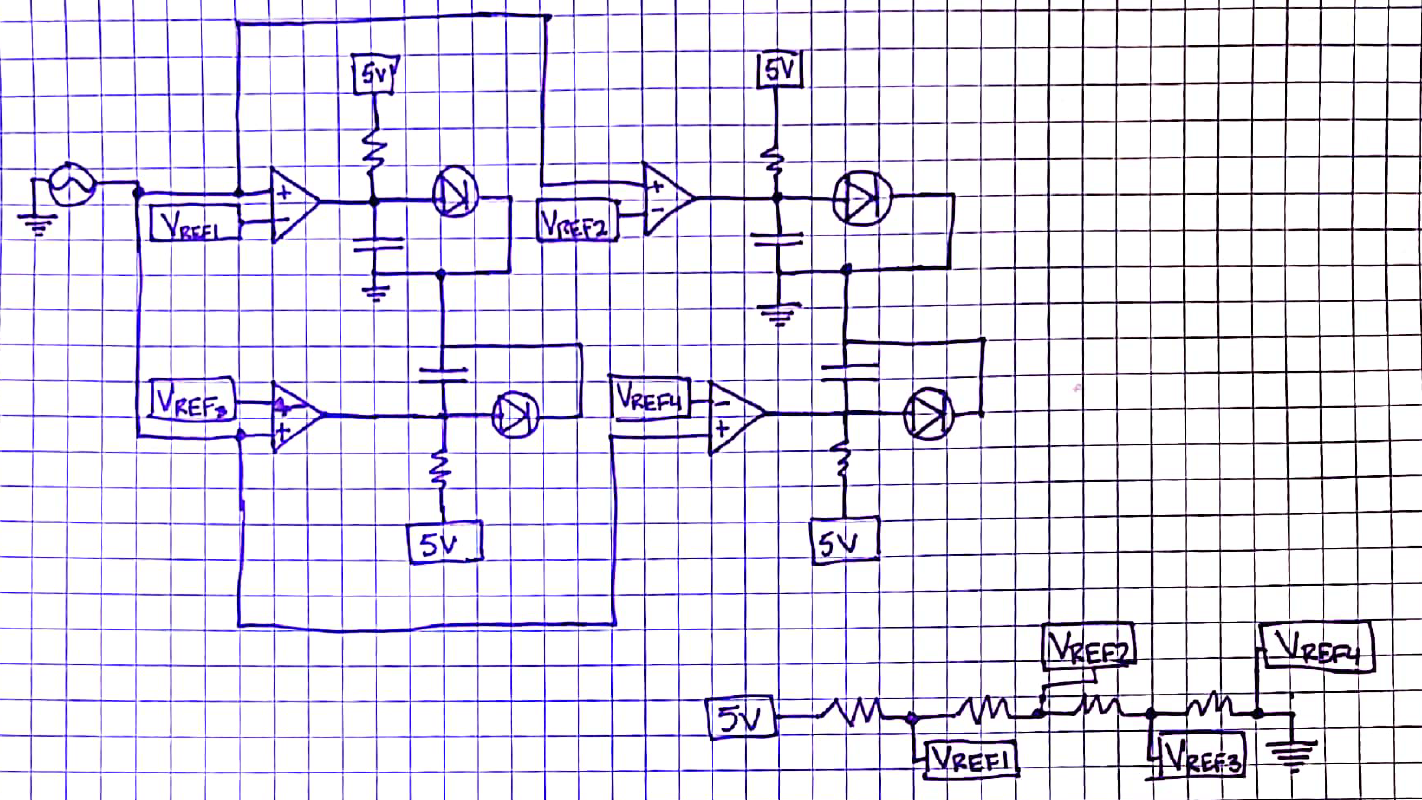
\includegraphics[width=5in]{fullSchem.png}
	\caption{Frequency and Gain Voltages}
	\label{fig1}
\end{figure}

\section{Analysis}
One arguable flaw of this system beyond efficiency is that our output is a shifting binary output rather than a straight binary output. When we increase a level of amplitude our output does increment binarily by one, but rather the right most least significant bit turns on. That gives only n+1 usable outputs, where n is the number of comparators (bits). A normal 4 bit output has $2^{4} = 16$ possible outputs, but we our only using $4+1=5$ of those outputs. This proves a not only another layer of poor efficiency but also implies the requirement for additional hardware to convert this output to a more useful format. It would certainly depend on the application, but this is arguably not the most ideal output format.

%\begin{thebibliography}{99}
% The numeral (here 99) in curly braces is nominally the number of entries in
% the bibliography. It's supposed to affect the amount of space around the
% numerical labels, so only the number of digits should matter--and even that
% seems to make no discernible difference.
%Not Requested
%\end{thebibliography}

\end{document}
